% ============================================================
% CHAPITRE 9
% ============================================================
\chapter{Résultats : qualité de détection mesurée}
\label{ch:resultats}

\section{Protocole}
La plateforme est évaluée comme une boîte noire, contre la vérité terrain
publiée par le producteur (figure~\ref{fig:protocole}). Une fraude injectée est
\emph{détectée} si une alerte de niveau MEDIUM ou plus, du type attendu,
partage au moins une transaction avec elle, ou porte sur l'un de ses comptes
clés (la mule, le pivot, la source ou la destination). Une alerte est
\emph{vraie} si elle correspond ainsi à au moins une fraude injectée. Seules
comptent pour le rappel les fraudes injectées au moins 8~minutes avant la
mesure, pour laisser au chemin lent le temps de passer.

\begin{figure}[htp]
\centering
\begin{tikzpicture}[
  b/.style={draw=#1, line width=0.9pt, fill=#1!8, rounded corners=3pt, align=center,
    font=\sffamily\scriptsize, minimum height=1.0cm, text width=2.6cm},
  f/.style={-{Stealth[length=1.9mm]}, line width=0.8pt, color=encre2}]
  \node[b=bleuprojet] (p) at (0,0) {\textbf{Producteur}\\{\tiny trafic + 1 fraude / 30 s}};
  \node[topic] (gt) at (3.4,1.0) {ground-\\truth};
  \node[topic] (tx) at (3.4,-1.0) {transactions};
  \node[b=orangeprojet] (s) at (6.8,-1.0) {\textbf{Plateforme}\\{\tiny boîte noire}};
  \node[b=orangeprojet, text width=2.2cm] (a) at (10.0,-1.0) {\textbf{alertes}\\{\tiny gold, $\geq$ MEDIUM}};
  \node[b=vertcode, text width=3.4cm, minimum height=2.9cm] (e) at (13.6,0) {\textbf{evaluate.py}\\[3pt]
    {\tiny \textbf{rappel} : fraudes détectées / fraudes injectées\\[2pt]
    \textbf{précision} : alertes vraies / alertes émises\\[2pt]
    \textbf{délai} : dernier virement de la fraude → première alerte du type attendu\\[2pt]
    \textbf{latence} : ingestion Kafka → alerte}};
  \draw[f] (p) |- (gt);
  \draw[f] (p) |- (tx);
  \draw[f] (tx) -- (s);
  \draw[f] (s) -- (a);
  \draw[f] (a) -- (a -| e.west);
  \draw[f, dashed] (gt) -- (gt -| e.west);
  \node[font=\sffamily\tiny, color=encre2] at (8.4,1.25) {jamais lue par les détecteurs};
\end{tikzpicture}
\caption{Protocole d'évaluation : la vérité terrain contourne la plateforme.}
\label{fig:protocole}
\end{figure}

\section{Rappel et précision}
Sur la période évaluée (29,5~minutes, 42~fraudes, 111~alertes), la plateforme
détecte \textbf{39 fraudes sur 42} et \textbf{101 de ses 102 alertes}
significatives correspondent à une fraude réelle (figure~\ref{fig:rp}). Toutes
les typologies sont détectées à 100\,\%, sauf les comptes mules
(12 sur 15). Deux des trois mules manquées ont été injectées dans les quatre
premières minutes après la chauffe, quand l'historique des comptes était
encore court. La seule fausse alerte est un cycle de niveau MEDIUM (score 40),
à la limite du seuil.

\aretenir{Ce que ces chiffres signifient}{Les données sont synthétiques : ces chiffres mesurent la
capacité de la plateforme à retrouver des schémas \emph{connus}, noyés dans un trafic réaliste, et non
sa performance sur de vraies fraudes, plus variées. Ils montrent en revanche trois choses solides :
la détection de forme fonctionne en flux, elle reste précise malgré les boucles fortuites du trafic
légitime, et chaque filtre de la chaîne a un effet mesuré.}

\begin{figure}[htp]
\centering
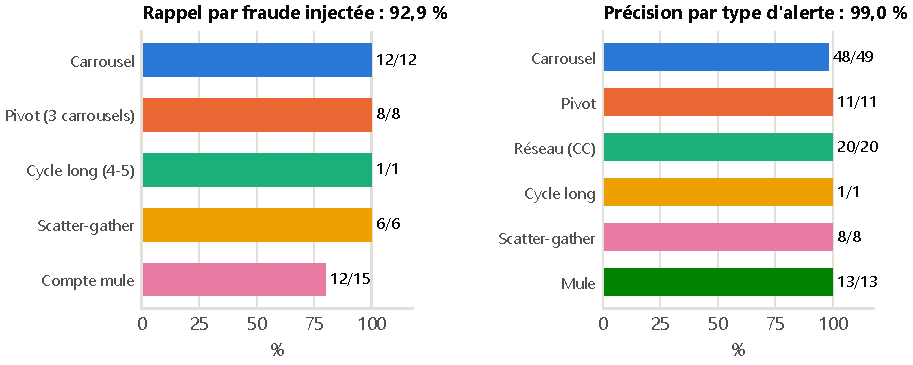
\includegraphics[width=\linewidth]{figures/rappel_precision.pdf}
\caption[Rappel et précision]{Rappel par typologie injectée (gauche) et précision par type d'alerte
(droite) sur le run d'évaluation final. Les alertes Réseau (CC) et Pivot reprennent des fraudes déjà
détectées comme carrousels : elles comptent pour la précision, pas pour le rappel.}
\label{fig:rp}
\end{figure}

\section{Délais de détection}
Le délai mesure le temps entre le \emph{dernier} virement d'une fraude --- le
moment où elle est complète --- et sa première alerte
(figure~\ref{fig:delais}). Les carrousels sont signalés en \textbf{3,9~secondes}
en médiane (8~secondes au maximum). Les autres typologies, analysées par le
chemin lent, le sont en une à deux minutes : la cadence de 90~secondes en
fixe l'ordre de grandeur. Les pivots sont signalés en 4,9~secondes en médiane
car leurs carrousels le sont dès qu'ils se ferment ; l'alerte PIVOT proprement
dite suit au passage du chemin lent.

\begin{figure}[htp]
\centering
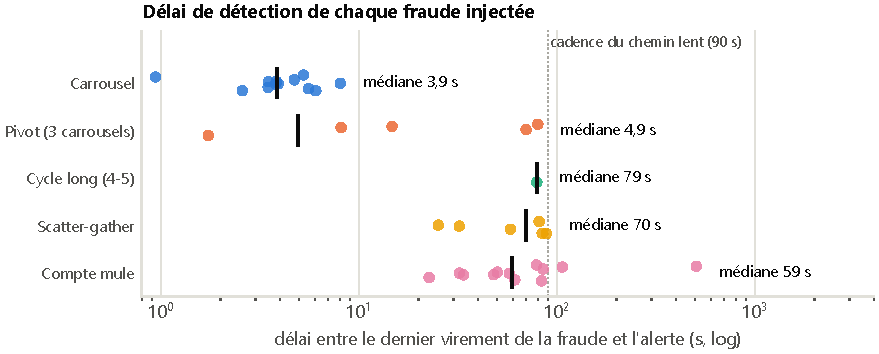
\includegraphics[width=\linewidth]{figures/delais_detection.pdf}
\caption[Délai de détection par typologie]{Délai de détection de chacune des 39 fraudes détectées
(échelle logarithmique) ; le trait noir marque la médiane.}
\label{fig:delais}
\end{figure}

\begin{figure}[htp]
\centering
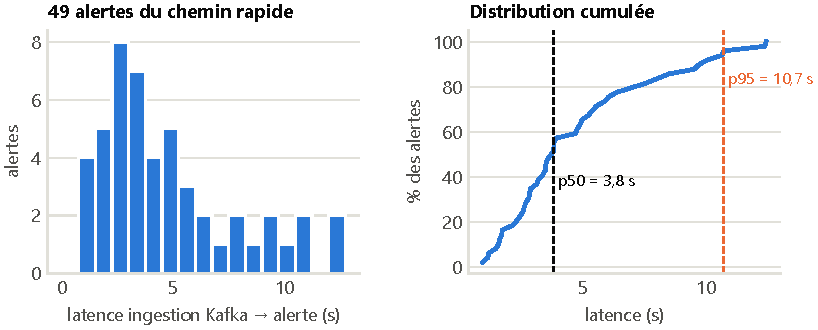
\includegraphics[width=\linewidth]{figures/latence_chemin_rapide.pdf}
\caption[Latence du chemin rapide]{Latence de bout en bout du chemin rapide, de l'ingestion de la
transaction par Kafka à la publication de l'alerte : p50 = 3,8~s, p95 = 10,7~s, p99 = 12,4~s.}
\label{fig:latence}
\end{figure}

\section{Ce qu'apporte chaque filtre : étude d'ablation}
Pour savoir si chaque étape de la détection est utile, la détection des
carrousels est rejouée hors ligne sur 90\,323 transactions d'un run
précédent, en ajoutant les filtres un à un (figure~\ref{fig:ablation}). Le
motif seul trouve 233 cycles, dont 165 boucles fortuites entre comptes très
actifs : 29\,\% de précision. L'ordre temporel élimine 142 de ces boucles
fortuites, le score 22 des 23 restantes. Aucun des 36 carrousels injectés
n'est perdu en route.

\begin{figure}[htp]
\centering
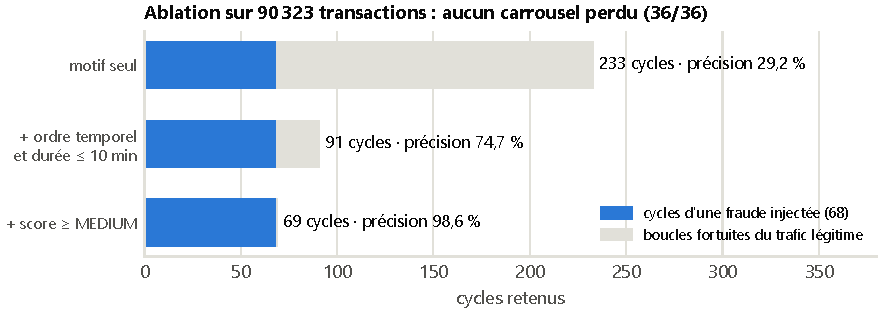
\includegraphics[width=\linewidth]{figures/ablation.pdf}
\caption[Étude d'ablation]{Étude d'ablation de la détection des carrousels
(\fichier{scripts/evaluate.py --ablation}).}
\label{fig:ablation}
\end{figure}

\section{Évolution au fil des runs}
Le run final est le cinquième run d'évaluation complet
(figure~\ref{fig:historique}). Le rappel a d'abord progressé avec la refonte
de la règle des mules (A → B), puis légèrement reculé quand la règle a été
rendue plus stricte pour éliminer les faux positifs de commerçants ; la
latence p95, elle, a révélé la fuite mémoire (C) avant d'être maîtrisée (E).

\begin{figure}[htp]
\centering
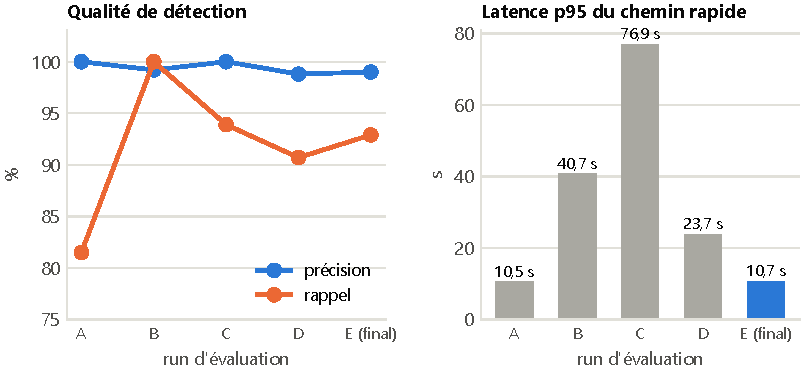
\includegraphics[width=\linewidth]{figures/historique_runs.pdf}
\caption[Cinq runs d'évaluation]{Cinq runs d'évaluation successifs. A : premier run complet ;
B : règle des mules révisée ; C : index d'adjacence et Arrow (fuite mémoire) ; D : libération
des checkpoints locaux ; E : mémoire native bornée (run final). Valeurs relevées dans
\fichier{docs/resultats.md} à chaque run.}
\label{fig:historique}
\end{figure}

\clearpage
\section{Synthèse}
Le tableau~\ref{tab:synthese} rassemble les indicateurs mesurés au fil de ce
chapitre et des précédents.

\begin{table}[h]
\centering\small
\begin{tabular}{@{}>{\raggedright\arraybackslash}p{6.2cm}>{\raggedright\arraybackslash}p{4.2cm}>{\raggedright\arraybackslash}p{3.6cm}@{}}
\toprule
\sffamily\bfseries Indicateur & \sffamily\bfseries Valeur & \sffamily\bfseries Source\\
\midrule
Précision des alertes ($\geq$ MEDIUM) & \textbf{99,0\,\%} (101 / 102) & run final\\
Rappel & \textbf{92,9\,\%} (39 / 42) & run final\\
\quad carrousels, pivots, cycles longs, scatter-gather & 100\,\% & \\
\quad comptes mules & 80\,\% (12 / 15) & \\
Délai de détection d'un carrousel & \textbf{3,9~s} médiane, 8,1~s max & run final\\
Latence du chemin rapide & 3,8~s (p50), 10,7~s (p95) & run final\\
Débit soutenu & 100~tx/s sans dérive & benchmark\\
Précision des carrousels : motif seul → final & 29\,\% → 99\,\% sans perte & ablation\\
Doublons après un arrêt brutal de Spark & \textbf{0} & test de panne\\
\bottomrule
\end{tabular}
\caption{Synthèse des résultats mesurés.}
\label{tab:synthese}
\end{table}
